\documentclass[../experiment.tex]{subfiles}
\graphicspath{{\subfix{../../../images/}}}
\begin{document}
    \textbf{Calcium Sodium Sulphate ($CaNa_2{(SO_4)}_2$)} consists of one calcium ion ($Ca^{2+}$) and two sodium 
    ions ($Na^+$) combined with two sulfate ions (${SO_4}^{2-}$). The calcium and sodium ions contribute to the 
    cationic structure, while the sulfate ions form the anionic part. It typically exists as a white crystalline 
    solid. It has a relatively high melting point and is sparingly soluble in water. The exact physical properties, 
    such as density and hardness, may vary depending on the specific crystalline form and conditions.Calcium 
    sodium sulfate is not commonly found in nature as a distinct mineral. However, it may form as a component in 
    certain mineral deposits or as a result of industrial processes. Due to its limited natural occurrence, 
    calcium sodium sulfate does not have significant industrial applications on its own. However, it may be used 
    as a source of calcium and sodium ions in various chemical processes or as an ingredient in specific 
    formulations. It can undergo various chemical reactions depending on the specific conditions. For example, it 
    can react with acids to release sulfuric acid and form corresponding salts. It can also participate in 
    precipitation reactions or form solid compounds with other ions.

    \subsubsection{Synthesis of $CaNa_2{(SO_4)}_2$ (pure)}
        Calcium Sodium Sulphate was prepared by chemical co-precipitation method\cite{a12}\cite{a13} using the following chemical reaction.
        \begin{center}
            \ce{2NaCl + CaCl_2 + 2(NH_4)_{2}SO_4 -> CaNa_2(SO_4)_2 + 4NH_{4}Cl}
        \end{center}
        To synthesize $CaNa_2{(SO_4)}_2$ 14.702g of $CaCl_2$ and 11.688g of $NaCl$ was added to 100ml of double-distilled
        water in a beaker and stirred continuously with a magnetic stirrer. Simultaneously a solution of 26.426g of
        ${(NH_4)}_{2}SO_4$ in 100ml double distilled water was prepared and added drop wise to the previous solution using a
        burette while being continuously stirred using a magnetic stirrer.A milky white precipitate was observed to be
        forming at the bottom of the beaker.

        The solution along with precipitate was then centrifuged 3\-4 times using a centrifuge and the precipitate
        thus obtained was separated and placed on a heating mantle at $40^{\circ}C$ for 2 hours and then the temperature was
        increased to $60^{\circ}C$ for the next 5 hours while finally increasing temperature to $80^{\circ}C$ and heating the sample for
        1 hour. The sample was then let to cool down to room temperature and then grounded into a fine powder using
        a mortar and pestle. The sample was then stored in a cool and dark place to be tested for its thermoluminescence
        properties.The sample was then taken to Inter University Accelerator Centre (IUAC) where it was annealed at
        constant temp of $400^{\circ}C$ in a muffle furnace for 2 hours and then bought back to room temperature to remove
        any previous radiation.
        \FloatBarrier\begin{multicols}{2}
            \begin{Figure}
                \centering
                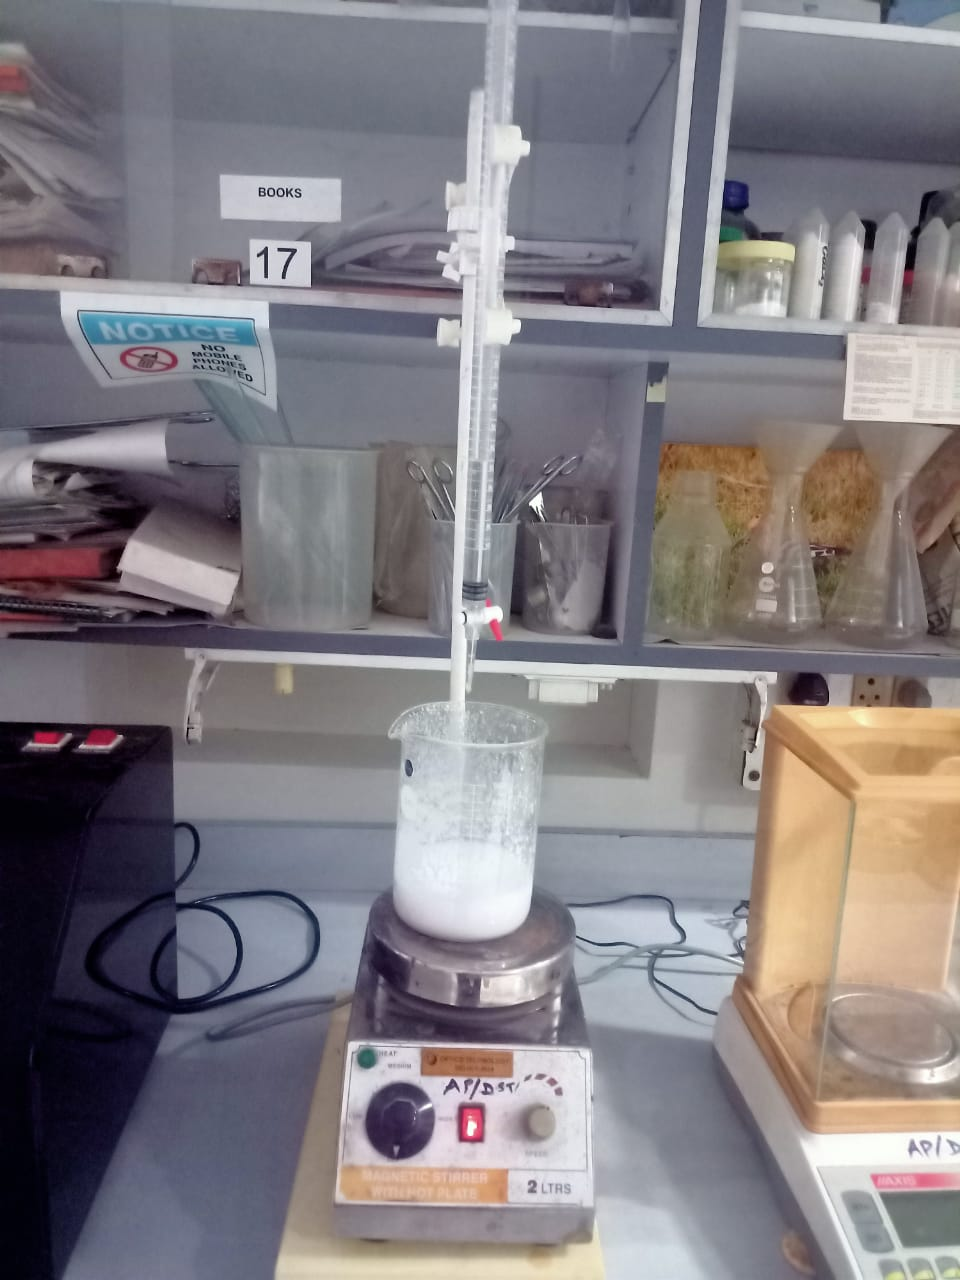
\includegraphics[width=0.5\linewidth]{pic1.jpg}
                \captionof{figure}{Formation of precipitate due to drop-wise addition of (NH$_4$)$_2$SO$_4$ to the solution}\label{fig:pic1}
            \end{Figure}
            \begin{Figure}
                \centering
                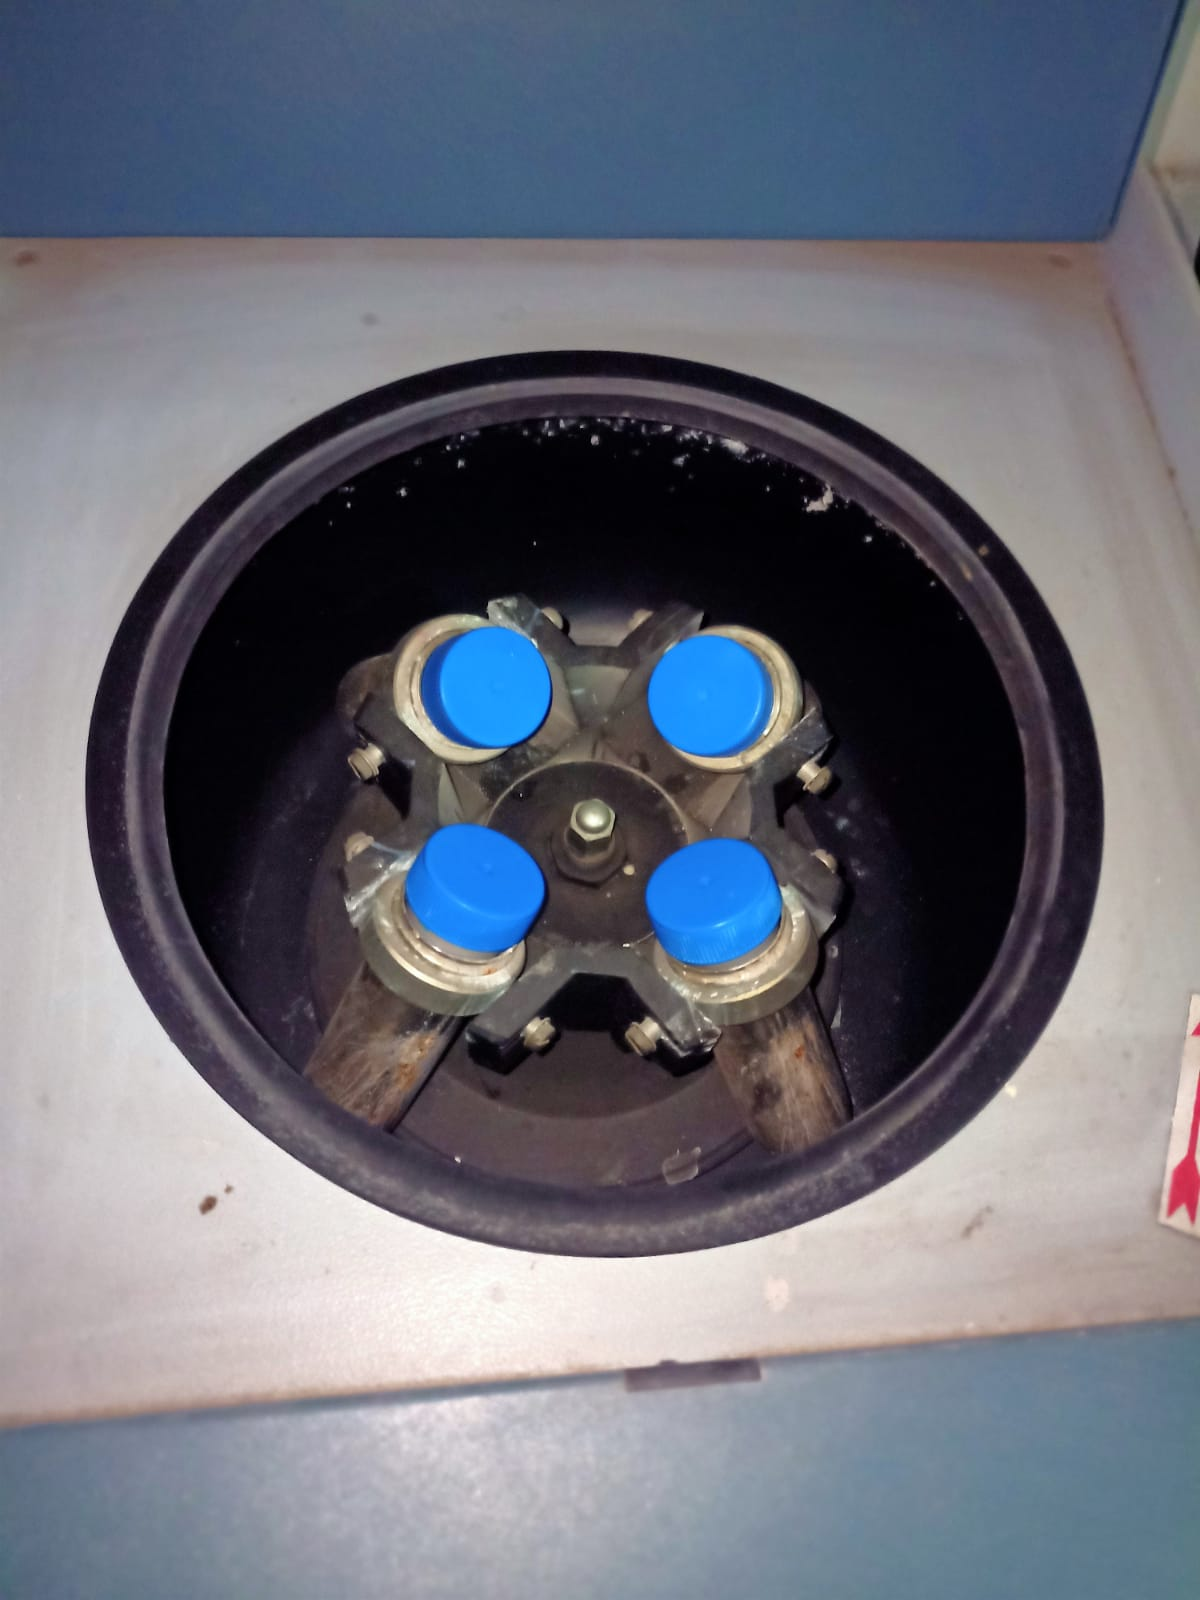
\includegraphics[width=0.5\linewidth]{pic2.jpg}
                \captionof{figure}{Centrifuging the sample}\label{fig:pic2}
            \end{Figure}
        \end{multicols}
    \subsubsection{Synthesis of $CaNa_2{(SO_4)}_2:Eu(0.1 mol\%)$}
        Calcium Sodium Sulphate doped with Europium was prepared by chemical co-precipitation method using the following chemical reaction.
        \begin{center}
        \ch{2 NaCl + CaCl_2 + 2 {(NH_4)}_{2}SO_4 -> [EuCl3. 6 H2O] CaNa_2{(SO_4)}_2:Eu + 4 NH_4Cl}
        \end{center}
        In a beaker with 100ml double distilled water 14.702g of $CaCl_2$ and 11.676g of $NaCl$ was added and stirred
        continuously with a magnetic stirrer. 0.0368g of $EuCl_{3}{\cdot}6H_2O$ was then added to the above solution and stirred
        continuously for 15 minutes. A solution of 26.426g of ${(NH_4)}_{2}SO_4$ in 100ml double distilled water was prepared
        and added drop wise to the above solution using a burette while being continuously stirred using a magnetic
        stirrer over a period of 3 hours.A milky white precipitate was observed to be forming at the bottom of the
        beaker. The solution along with precipitate was then centrifuged 3\-4 times using a centrifuge.

        The precipitate thus obtained was separated and placed on a heating mantle at $40^{\circ}C$ for 2 hours and then
        the temperature was increased to $60^{\circ}C$ for the next 5 hours while finally increasing temperature to $80^{\circ}C$ and
        heating the sample for 1 hour. The sample was then let to cool down to room temperature and then grounded
        into a fine powder using a mortar and pestle.Approximately 22g of powdered sample was obtained using this
        method. The sample was then stored in a cool and dark place to be tested for its thermoluminescence
        properties.The sample was then taken to Inter University Accelerator Centre (IUAC) where it was annealed at
        constant temp of $400^{\circ}C$ in a muffle furnace for 2 hours and then bought back to room temperature to remove
        any previous radiation.
        \FloatBarrier\begin{multicols}{2}
            \begin{Figure}
                \centering
                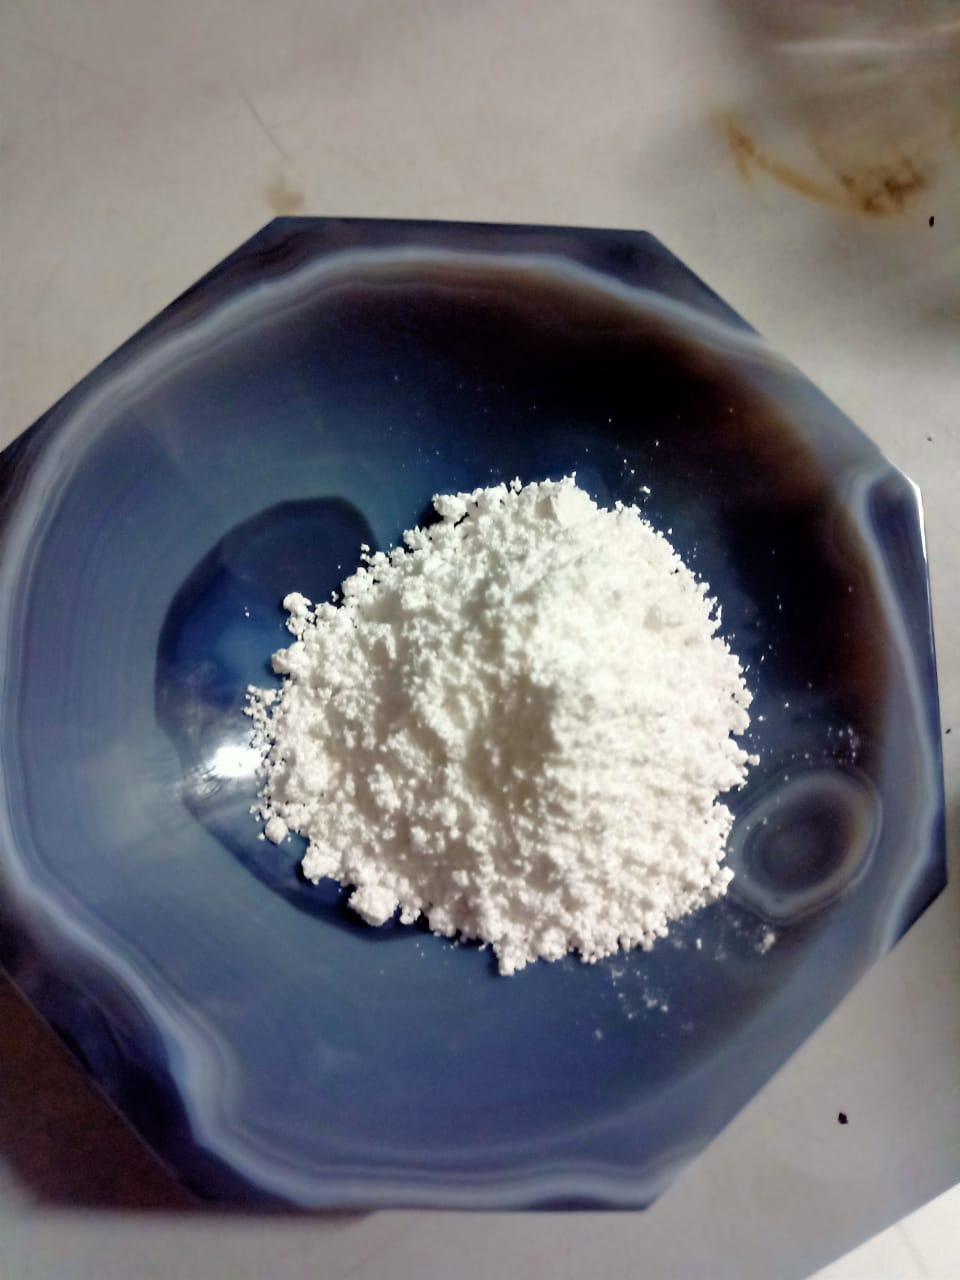
\includegraphics[width=0.6\linewidth]{pic3.jpg}
                \captionof{figure}{Sample grounded to a fine powder}\label{fig:pic3}
            \end{Figure}
            \begin{Figure}
                \centering
                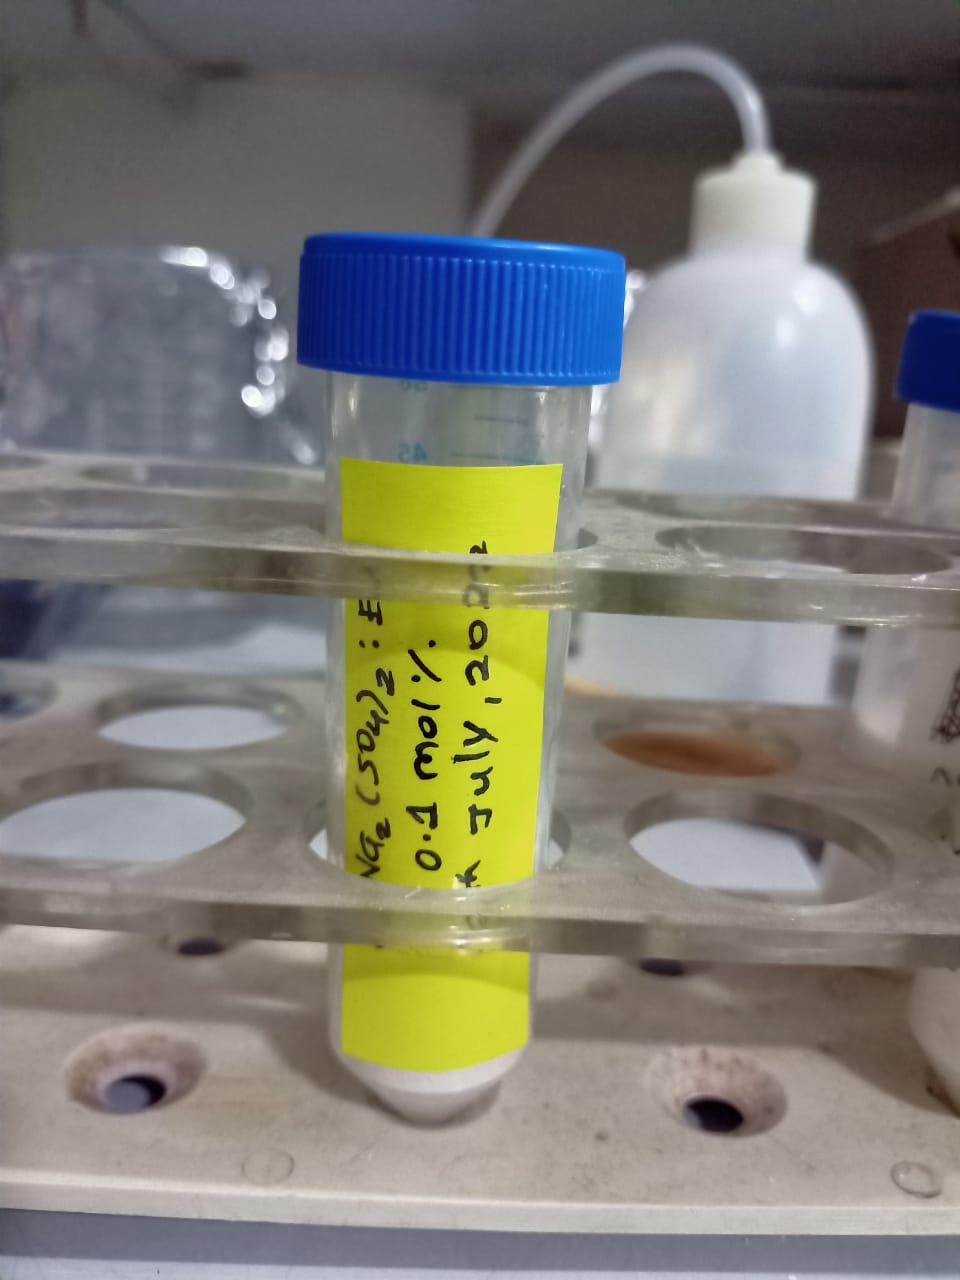
\includegraphics[width=0.6\linewidth]{pic4.jpg}
                \captionof{figure}{Final sample}\label{fig:pic4}
            \end{Figure}
        \end{multicols}
\end{document}